\section{Datos a analizar}

Los datos a analizar se tratan de opiniones sobre películas de la base de datos IMDb. La información de la que disponemos es de un identificador, la URL de la opinión, el texto que conforma la opinión e información sobre si la opinión es positiva o negativa.

En nuestro caso utilizaremos el texto como documento y el identificador para realizar operaciones sobre los datos y mantener la coherencia al realizar algunas operaciones sobre los datos.

\section{Lectura de los datos}



\section{Preprocesamiento para clasificación}



\section{Uso de métodos de clasificación}



\section{Uso de diccionarios para análisis de sentimientos}

\subsection{Lectura de diccionarios}

\subsection{Uso para decidir el sentimiento de documentos}


\section{Workflow final}


El flujo final realizado a lo largo de la práctica es el siguiente:

\begin{figure}[H]
	\centering
	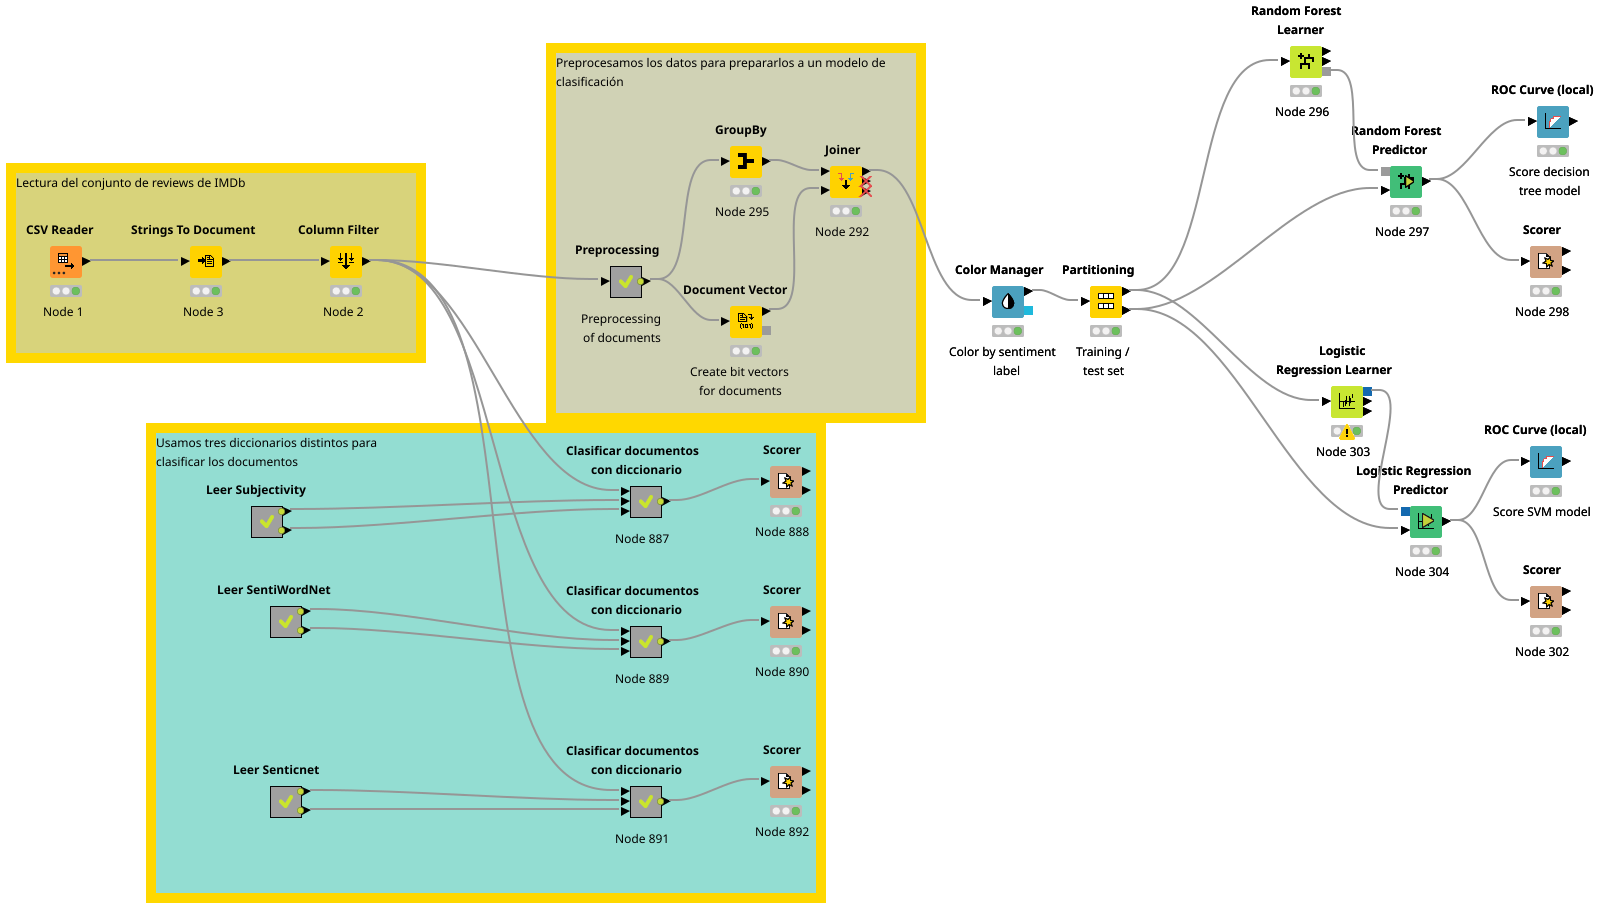
\includegraphics[width = \textwidth]{workflow_knime.png}
	\caption{Workflow final de KNIME.}
	\label{fig:workflow_knime}
\end{figure}
